
% --------------------------------
\section{Package Diagram}
The package diagram shows how the Heat Production Optimization system is organized by breaking the application into separate modules, each with its own specific tasks. The system is made up of different parts: the Asset Manager, the Source Data Manager, the Optimizer, the Result Data Manager, and the Data Visualization components.\par

The Asset Manager takes care of keeping fixed information about the heating grid and production units, while the Source Data Manager deals with changing data like heat demand and electricity prices. The Optimizer is the main part of the system. It takes information from both managers to figure out the best and most cost-effective plan for producing heat. Once the calculations are done, the results are saved in the Result Data Manager and shown to the user using the Data Visualization module.\par

All parts of the system are linked to a common storage area that uses CSV and JSON. This setup lets the system access input data and store the results of optimizations. This package layout was selected because it clearly distinguishes between how data is managed, the logic for optimization, and how information is presented. Because of this, the system is simpler to understand, easier to take care of, and can be updated with new features in the future. It is relevant because it explains the system’s structure, the role of each module, and the data flow, helping to understand and justify the design shown in the package diagram. 
\begin{figure}[H]
    \centering
    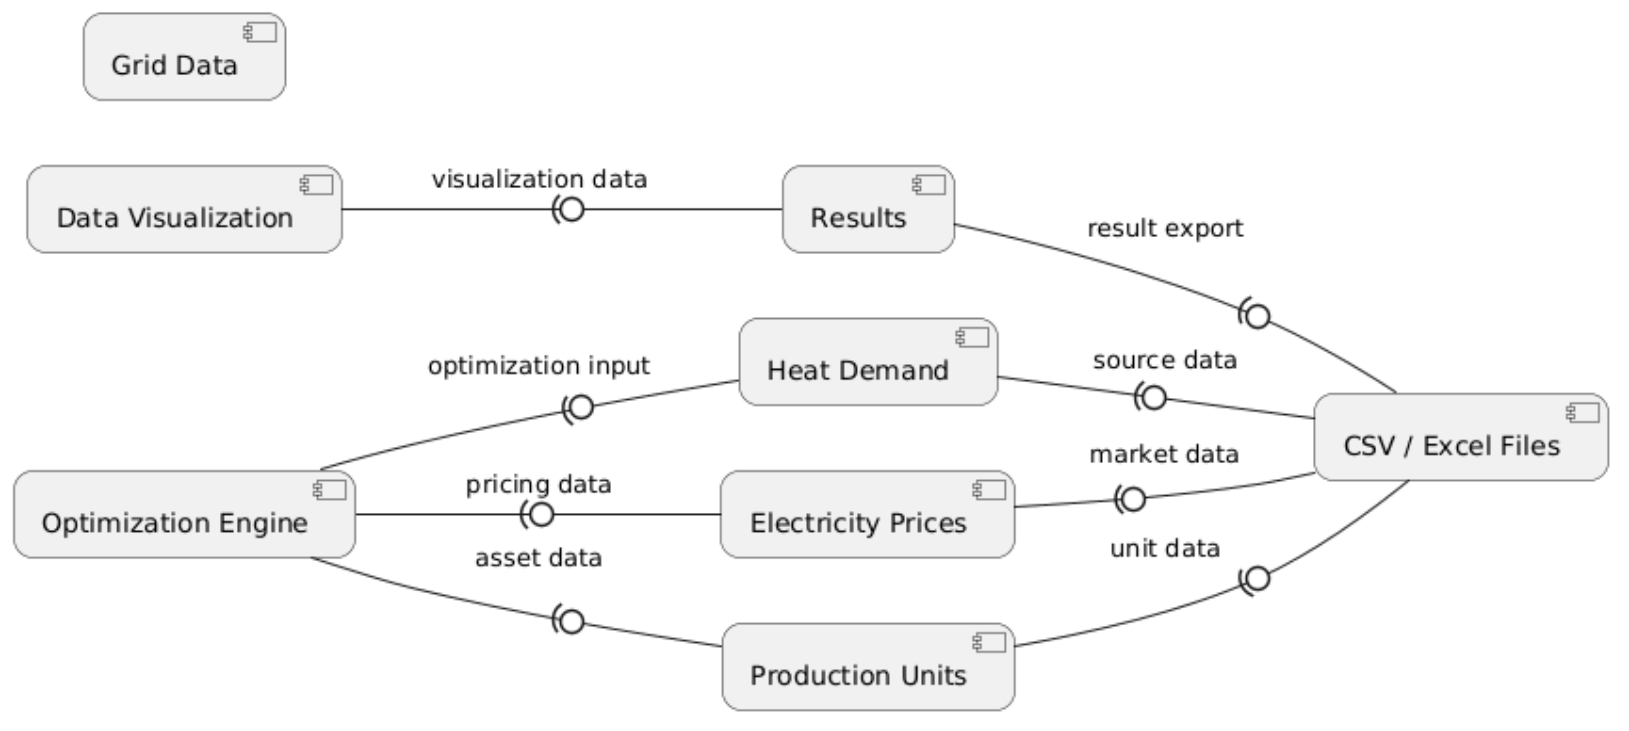
\includegraphics[width=0.75\textwidth]{Figures/Diagrams/PackageDiagram.png}
    \caption{Package Diagram}
    \label{fig:sprint-1-planning}
\end{figure}

% --------------------------------
\section{Class Diagram}
The diagram shows a system made up of different parts, with the Data Manager acting as the main one that brings everything together. It links the main parts - Asset Manager (AM), Source Data Manager (SDM), and Result Data Manager (RDM) - and takes care of important tasks like starting up the system, bringing in data, doing the optimization process, changing the selected time period, and sharing the results.\par

The AM is in charge of handling assets and scenario details. It stores a collection of Asset objects, which have details such as capacity, costs, and emissions, along with ScenarioData that sets priorities and maintenance rules. The SDM handles input data that changes over time using SourceData objects, which keep track of information like timestamps, heat demand, and electricity prices. The RDM is responsible for handling the output data (ResultData), including both summary statistics and detailed results. The data is generated by the Optimizer and can also be exported for further use.\par

The Optimizer uses information from AM and SDM to do calculations, like looking at costs and making plans for production. Additional parts such as ScenarioLoader and JSONPersistence help manage data by allowing the process of loading and saving information.\par

In short, the Data Manager connects all parts of the system together. Each manager handles a specific type of data. The Optimizer uses this data to create results, which are then viewed and shown through the ViewModels.\par

This design is relevant because it separates responsibilities between components, making the system easier to maintain and extend. Each manager focuses on a specific type of data, while the Data Manager coordinates the workflow. This clear structure improves scalability, simplifies updates, such as changing data sources or optimization logic, and ensures that results can be efficiently processed and reused. 
\begin{figure}[H]
    \centering
    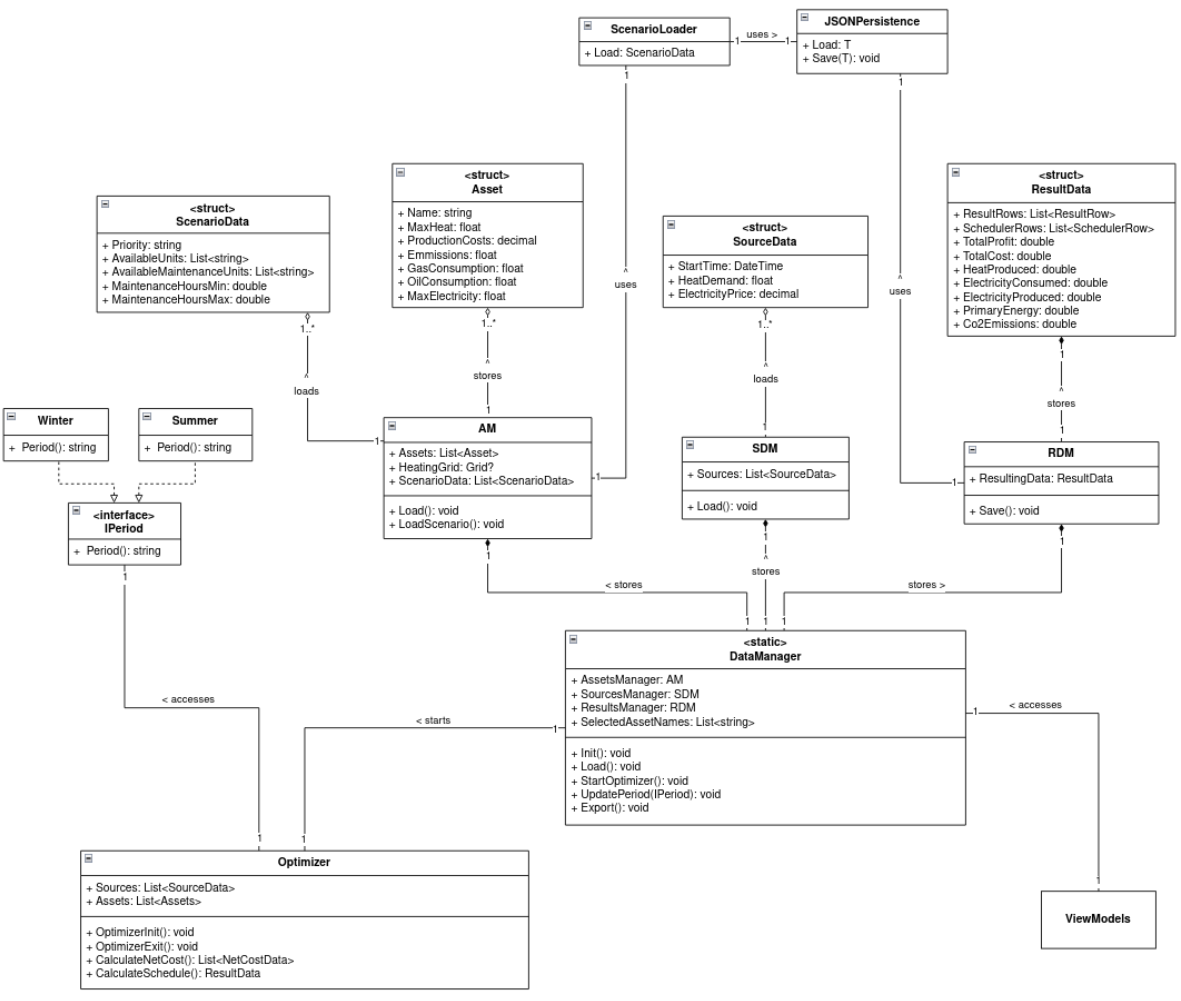
\includegraphics[width=0.75\textwidth]{Figures/Diagrams/ClassDiagram.png}
    \caption{Class Diagram}
    \label{fig:sprint-1-planning}
\end{figure}

% --------------------------------
\section{Activity Diagram}

The activity diagram represents the user interaction flow with the heat optimization system. The user begins with choosing the desired scenario followed by the heating period. Then, he or she can either proceed to edit production units or directly to the execution of the optimizer. After the system calculates the results, the user can export the data, view the charts or exit the program. The decision paths shown on the diagram represent the flexibility of the flow as the user can revisit earlier steps.\par
The diagram models the optimization execution process from the perspective of the user, rather than low-level implementation. Therefore, it provides a clear and intuitive representation of the workflow, which can be used to communicate the system behaviour to non-technical readers or stakeholders. Moreover, the diagram is used as a validation of the business objectives and high-level requirements, and to provide documentation for future maintenance.\par
Actions and the flow presented on the diagram connect to the implementation of UI functions and how user actions trigger system events. The support of loading pre-configured scenarios allows the user to run the optimization right after selecting the scenario and heating period, without the need to edit the units. The optimization and production units’ configuration pages are separate, and they can be accessed at any time. Once the optimization is started by pressing the Run Optimization button, the charts are updated with new data, and the export button becomes enabled.


\begin{figure}[H]
    \centering
    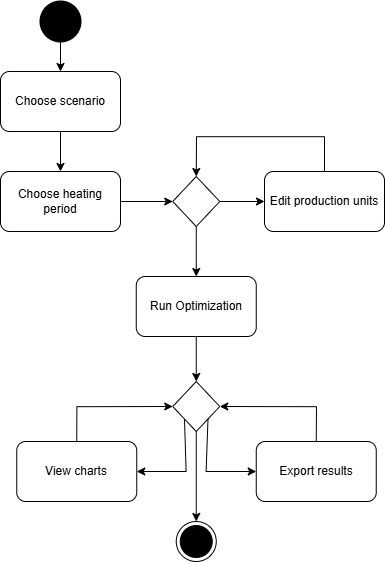
\includegraphics[width=0.75\textwidth]{Figures/Diagrams/ActivityDiagram.png}
    \caption{Activity Diagram}
    \label{fig:sprint-1-planning}
\end{figure}

% --------------------------------
\section{Sequence Diagram}
In this case, the process starts when the user sets up a scenario and chooses the right assets using the ViewModels, which then starts the system setup through the Data Manager. The Data Manager gets the necessary information by getting asset details from the Asset Manager and gathering time-related data, like demand and price, from the Source Data Manager. Once all the needed data is ready, the optimization process starts, and the prepared inputs are sent to the Optimizer.\par
The Optimizer goes through each time step one by one, getting the needed demand and price information. For each asset, it figures out the costs needed to produce it, sorts the assets by how efficient they are economically, and finds the best way to assign production while following the rules of how the operations work. Once the optimization is done, the results are collected and saved by the Result Data Manager. When the user asks for them, the results are sent back to the ViewModels, and then they are shown using things like charts and key performance indicators. This design was chosen to separate data management, optimization and presentation into distinct components. This is relevant because it creates a clear workflow, improves maintainability, and makes it easier to handle complex optimization results efficiently.


\begin{figure}[H]
    \centering
    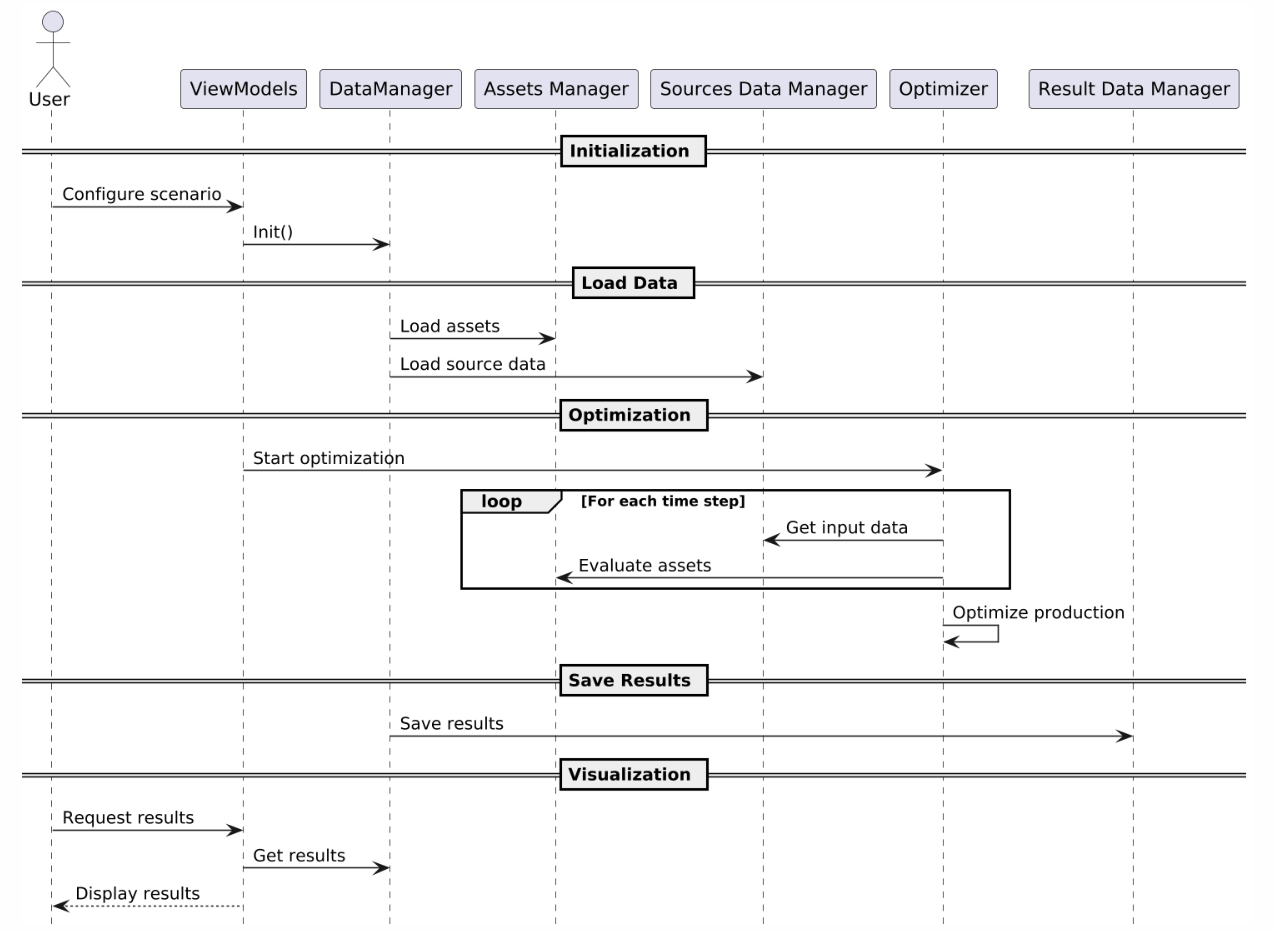
\includegraphics[width=0.75\textwidth]{Figures/Diagrams/SequenceDiagram.png}
    \caption{Sequence Diagram}
    \label{fig:sprint-1-planning}
\end{figure}

% --------------------------------
\section{Overall Technical Architecture}
\subsection*{Technology Stack}
Our technology stack for 2nd semester project was C\# for all frontend and backend, C\# Avalonia framework for frontend with data bindings, LiveCharts for data visualization, and NUnit for testing. Working with Avalonia proved to be more challenging than expected as online resources, documentation were not as high-quality and satisfactory as expected. Provided abstractions by Avalonia and their suggested design patterns did not allow for scaling code well while keeping codebase clean - data duplication, minor hacks for reactivity and passing data were required to achieve desired result and many of their official examples introduced substantial complexity. Additionally, LiveCharts library was limiting because it had issues with crashing outside of C\# code. For loading, storing and exporting state, JSON files were used. Due to small project scope, low volume of data, high flexibility, easier data management and the project being a standalone desktop application, storing data in JSON was more fit for the task than using traditional relational databases such as PostgreSQL or MySQL. The team have considered using Docker to standardize our development environment even further but the team have rejected it because there were no major issues of the application not working as expected on a different computer. There was only one issue during sprint 1 related to different path handling on Windows and Linux but it was fixed quickly. Furthermore, team members have considered integrating CI to our GitHub for running tests automatically but it was ruled out as unnecessary because during our code reviews reviewers already run tests among other review tasks and there would be no increase in development velocity from such integration at such project size.

\subsection*{Seperation of Concerns}
To keep our codebase clean, make it modular, easier to work with, and collaborate, 3-layer programming was used - application was split to presentation, domain and data layers. Additionally, the application was segmented into 5 modules. Asset Manager (AM) responsible for loading static data, Source Data Manager (SDM) responsible for loading dynamic data, Result Data Manager (RDM) for storing result data and exporting. They belonged to the data layer. Optimizer (OPT) responsible for considering all available data, scheduling available units optimally to reduce costs and scheduling units for maintenance, and Data Manager (DM) which connects the data layer to be accessible to the Optimizer module and the presentation layer. Data Manager acts as a thin wrapper around the data layer for the Data Visualization module to access it and for Optimizer it provides wrapper methods to call. These 2 modules belong to the domain layer. The Data Visualization (DV) module forms the entire part of the presentation layer. It is the single largest module and it is further broken down to different views and respective view models. Different tab groups are different views such as vertical scenario tab group and upper page tab group. Each different page tab is a different view, such as overview, optimizer and production units page. Smaller elements such as different graphs and edit production unit popup have their own views. Splitting data visualization to many different views proved helpful for readability, reuse and reducing merge conflicts.

\subsection*{Architecture and Rationale}
3-layer programming architectural pattern was implemented as our foundation for the codebase. In the Data Visualization module, each view had their respective view model with data bindings and commands, and it followed MVVM design pattern. The decision was made to choose MVVM over other GUI architectural patterns because it increases readability, reduces boilerplate, and reduces code complexity as long as only simpler Avalonia features were used. To keep GUI reactive to data changes, the observer pattern was used. Whenever data updates, a message is sent notifying that refresh is required and GUI components subscribe to the channel. Observer pattern looked like a perfect candidate for the task because it is heavily used in GUI development, is tried and tested, and keeps single responsibility principle with no significant downsides. However, due to the difficulty of passing events to components, only some parts of the code use observer pattern. Data Manager module which connects different modules acts as a singleton by using C\# static members.\par
Our code follows DRY principle of not repeating code by using modules and utility classes. The benefit of improved readability was a decisive choice. However, some Avalonia components were proven to be difficult to cleanly refactor to proper modular components without adding significant complexity. Furthermore, the codebase follows YAGNI principle of not having unnecessary code which is unused. Quite a few parts of our codebase were refactored and removed during the development which were not needed anymore or a better, more simple approach was found. SOLID principles were partially adhered to. Single responsibility is used heavily by splitting many features into different modules and classes. For Object-Oriented Programming class design, composition over inheritance was heavily used. Various edge cases of inheritance such as diamond problem and potential complex situations later down the line deterred us from using inheritance and composition had no drawbacks in our case. None of the classes besides the Data Visualization module use inheritance which only inherit Avalonia base classes to implement functionality. As such, Liskov substitution principle is upheld. Open-closed principle is partially followed, as due to heavy use of composition, changing related classes can extend the behavior of the classes without modification but there are no specific mechanisms beyond composition to allow extending class functionality without modification. Interface segregation principle and dependency inversion principle were not strictly adhered to because there is only one interface in the codebase. Instead, composition on concrete classes were used. Decision was made to follow KISS principle to keep simplicity instead of introducing additional abstraction layers using interfaces. In such a relatively small project, additional simplicity and reduced boilerplate allowed for quicker iteration.

  
